\documentclass[9pt,twocolumn,twoside]{gsag3jnl}

\usepackage{subcaption}
\usepackage{multirow}
\usepackage{color,xcolor,xspace}
\newcommand{\N}{\text{N}}
\newcommand{\twolinecell}[2][c]{%
  \begin{tabular}[#1]{@{}c@{}}#2\end{tabular}}
\graphicspath{{images/}}

\newcommand{\redstar}{\textcolor{red}{*}}

\newcommand{\E}{\text{E}}
\newcommand{\V}{\text{V}}

\newcommand{\LM}{LM\xspace}
\newcommand{\Lev}{Levene's test\xspace}

\newcommand{\Caom}{Cao\textsubscript{M}\xspace}
\newcommand{\Caov}{Cao\textsubscript{V}\xspace}
\newcommand{\Caomv}{Cao\textsubscript{MV}\xspace}

\newcommand{\DGLMm}{DGLM\textsubscript{M}\xspace}
\newcommand{\DGLMv}{DGLM\textsubscript{V}\xspace}
\newcommand{\DGLMmv}{DGLM\textsubscript{MV}\xspace}

\newcommand{\gAA}{\text{AA}}
\newcommand{\gAB}{\text{AB}}
\newcommand{\gBB}{\text{BB}}


\newcommand{\FPR}{\text{FPR}}

\newcommand{\beginsupplement}{%
        \setcounter{table}{0}
        \renewcommand{\thetable}{S\arabic{table}}%
        \setcounter{figure}{0}
        \renewcommand{\thefigure}{S\arabic{figure}}%
        \FloatBarrier
		\onecolumn
     }
     
% \definecolor{vlow}{rgb}{0.6,0.6,0.95}
% \definecolor{low}{rgb}{0.8,0.85,0.95}
% \definecolor{good}{rgb}{1,1,1}
% \definecolor{high}{rgb}{0.95,0.8,0.75}
% \definecolor{vhigh}{rgb}{0.95,0.6,0.6}

% \definecolor{poorpower}{RGB}{245, 225, 220}
% \definecolor{okaypower}{RGB}{245, 200, 195}
% \definecolor{goodpower}{RGB}{245, 175, 170}
% \definecolor{highpower}{RGB}{245, 150, 145}
% \definecolor{vhighpower}{RGB}{245, 130, 125}
% \definecolor{toppower}{RGB}{245, 110, 105}

\definecolor{power}{rgb}{1, 1, 1}

\renewcommand{\b}{\textbf}
\renewcommand{\u}{\uline}
\newcommand{\uu}{\uuline}


\def\dout{\bgroup
 \markoverwith{\lower-0.2ex\hbox
 {\kern-.03em\vbox{\hrule width.2em\kern0.45ex\hrule}\kern-.03em}}%
 \ULon}
\MakeRobust\dout

\newcommand{\WV}[2]{\textcolor{red}{#1\footnote{\textcolor{red}{WV: #2}}}}
\newcommand{\RC}[2]{\textcolor{purple}{#1\footnote{\textcolor{purple}{RC: #2}}}}
\newcommand{\WVinline}[1]{\textcolor{red}{#1}}
\newcommand{\WVst}[1]{\textcolor{red}{\st{#1}}}
\newcommand{\reply}{\ensuremath{\hookrightarrow}\xspace}
\newcommand{\AddRefs}[1]{\textcolor{purple}{(Add refs: #1)}}
\newcommand{\DRAFT}[1]{\textcolor{darkgray}{DRAFT: #1}}
\newcommand{\CortyRPaper}{\textcolor{purple}{Corty and Valdar 2018+ [r/vqtl]}\xspace}
\newcommand{\CortyReanalysisPaper}{\textcolor{purple}{Corty \emph{et al} 2018+}\xspace}
\newcommand{\CortyMethodsPaper}{\textcolor{purple}{Corty and Valdar 2018+ [BVH]}\xspace}
 
\newcommand{\eg}{\emph{e.g.}\xspace}
\newcommand{\ie}{\emph{i.e.}\xspace}
\newcommand{\etal}{\emph{et al.}\xspace}
\newcommand{\indicator}[1]{I_{\left\{ {#1} \right\}}}
\newcommand{\indep}{\ensuremath{\perp\mkern -10mu \perp}}
\newcommand{\notindep}{\ensuremath{\perp\mkern -10mu \perp \mkern -16mu \not \mkern 16mu}}
\newcommand{\T}{^\mathrm{T}}
\newcommand{\Norm}{\mathrm{N}}
\newcommand{\veps}{\varepsilon}
\newcommand{\balpha}{\boldsymbol{\alpha}}
\newcommand{\bbeta}{\boldsymbol{\beta}}
\newcommand{\btheta}{\boldsymbol{\theta}}
\newcommand{\bveps}{\boldsymbol{\varepsilon}}
\newcommand{\bc}{\mathbf{c}}
\newcommand{\bd}{\mathbf{d}}
\newcommand{\bq}{\mathbf{q}}
\newcommand{\by}{\mathbf{y}}
\newcommand{\bx}{\mathbf{x}}
\newcommand{\bz}{\mathbf{z}}
\newcommand{\Expect}{\text{E}}
\newcommand{\Var}{\text{Var}}
 
\newcommand{\Table}[1]{\textbf{Table}~#1\xspace}
\newcommand{\Figure}[1]{\textbf{Figure~#1}\xspace}
\newcommand{\Eq}[1]{\textbf{Eq}~#1\xspace}


\articletype{inv} % article type

\title{\texttt{vqtl}: An \texttt{R} package for Mean-Variance QTL Mapping}

\author[$\ast$,1]{Robert W. Corty}
\author[$\ast, 1$]{William Valdar}

\affil[$\ast$]{University of North Carolina at Chapel Hill, Department of Genetics}

\keywords{QTL mapping, vQTL, mvQTL, variance heterogeneity, DGLM, R}

\runningtitle{Package vqtl} % For use in the footer 

\runningauthor{Corty and Valdar}

\graphicspath{{./images/}}


\begin{abstract}
We present \texttt{vqtl}, an \texttt{R} package for mean-variance QTL mapping.
This QTL mapping approach tests for genetic loci that influence the mean of the phenotype, termed mean QTL, the variance of the phenotype, termed variance QTL, or some combination of the two, termed mean-variance QTL.
It is unique in its ability to correct for variance heterogeneity arising not only from the QTL itself but also from nuisance factors, such as sex, batch, or housing.
This package provides functions to conduct genome scans, run permutations to assess the statistical significance, and make informative plots to communicate results.
Because it is inter-operable with the popular \texttt{qtl} package and uses many of the same data structures and input patterns, it will be straightforward for geneticists to analyze future experiments with \texttt{vqtl} as well as re-analyze past experiments, possibly discovering new QTL.
% % Mean-variance QTL mapping, a relatively novel approach to QTL mapping, elevates phenotype variance to the same level of consideration as phenotype mean.
% Most existing methods for QTL mapping in experimental crosses assume that the residual variance is constant across all individuals.
% But common situations violate this assumption.
% For many phenotypes, one sex is more variable than the other, some experimenters make more precise measurements than others, and specific genetic factors influence environmental sensitivity.
% In these cases, mean-variance QTL mapping provides higher power and better protection against false positives.
% It also allows for detection of QTL that influence phenotype variance, termed vQTL and QTL that influence some mixture of phenotype mean and variance, termed mvQTL.
% We present \texttt{R} package \texttt{vqtl}.
% This package makes it easy for geneticists to apply the mean-variance QTL mapping approach, control family-wide error rate (FWER), and visualize and interpret their results.
\end{abstract}

\setboolean{displaycopyright}{true}



% \linespread{2}

\begin{document}

\maketitle
\thispagestyle{firststyle}
\logomark
\articletypemark
\marginmark
\firstpagefootnote
\correspondingauthoraffiliation{Correspondence e-mail: william.valdar@unc.edu}
\vspace{-24pt}%



\section*{Introduction}

QTL mapping studies in experimental crosses have provided important insights on nearly every trait of interest in human health, as well as livestock and crop improvement programs.
Advances in model organism genotyping \citep{Williams1990} and phenotyping \citep{Yang2014a} as well as in statistical methods \citep{Lander1989a,Martinez1992} and software tools (\eg, \citealt{Broman2003,Mulligan2017}) have supported these discoveries.

It has long been recognized that the extent of residual variation is itself a heritable trait \citep{Falconer1965,Lynch1998}.
This phenomenon has been described theoretically \citep{Hill2004-uo,Hill2010} and demonstrated in inbred model organisms \citep{Sorensen2015,Ayroles2015} and crops \citep{Yang2012-aw,Forsberg2015} and exploited in livestock improvement efforts \citep{Mulder2008,Ibanez-Escriche2008-ie}.

However, traditional QTL mappinng analyses have focused on discovering ``mean QTL'', regions of the genome where allelic variation drives heterogeneity of phenotype mean, while assuming that the residual variance, that is, the intrinsic stability or noisiness of the phenotype, is identical for each every individual in the mapping population.
Recent work, however, has challenged the assumption of homogeneous variance and sought to identify an additional type of QTL --- those that
%, by driving heterogeneity of epistatic or environmental variance, 
influence the extent of residual variance, sometimes termed ``variance QTL'' (vQTL) \citep{Pare2010,Ronnegard2011a,Ronnegard2012,Cao2014}.

Although detection of vQTL has started to enter the mainstream of genetic analysis \citep{Yang2012,Hulse2013,Ayroles2015,Wei2016-lt,Wang2017,Wei2017-tt}, the statistical methods used for this purpose remain heterogeneous.
% and sometimes idiosyncratic, with connections to methods for mapping mean QTL often lacking or unclear.
% a clear or intuitive connection to methods used for detecting mean QTL.
%there remains great heterogeneity among the statistical methods used to conduct these analyses.
We developed a standardized method for QTL mapping that can detect mQTL, vQTL, and a generalization of the two that we term ``mvQTL''.
This approach, which we term ``mean-variance QTL mapping'', can be applied to intercross and backcross designs.
In two companion articles, we characterize this method and competitors in the setting where a background factor drives variance heterogeneity (\CortyMethodsPaper), and use it to discover new QTL from two existing data resources (\CortyReanalysisPaper)

Here, we provide a practical guide to using the \texttt{R} package \texttt{vqtl}, which implements mean-variance QTL mapping.
First, to generate illustrative data, we simulate an F2 intercross and four phenotypes: one phenotype determined entirely by random noise, and one with each of the three kinds of QTL.
On each phenotype we then conduct a genome scan using standard approximations to interval mapping \citep{Lander1989a,Martinez1992}, and mean-variance QTL mapping, which includes a test for mQTL, a test for vQTL, and a test for mvQTL.
The association statistics of all four tests are then initially plotted in LOD score units, with drawbacks of this plotting unit discussed.
Permutation scans are used to determine empirically adjusted $p$-values, and plotting in these units is shown to to make the results of the four tests more comparable.
Last, we describe plots to communicate the effects that led to the detection of a QTL, and use the bootstrap to estimate its confidence interval.

In two companion articles, we apply mean-variance QTL mapping with package \texttt{vqtl} to discover new QTL.
In the first, we describe a novel vQTL for exploratory behavior and a novel mQTL for a circadian behavior trait, both in mouse F2 intercrosses retrieved from the Mouse Phenome Database (\CortyReanalysisPaper) \citep{Bogue2015}.
The dataset from one of these intercrosses is used to benchmark the performance of package \texttt{vqtl}, as is described in the ``Performance Benchmarks'' section.
In the second, we describe a unique strength of mean-variance QTL mapping, its ability to accommodate variance heterogeneity arising from background factors, such as sex, batch, and housing, and demonstrate the value of such accommodation with both simulation studies and a report of a novel QTL (\CortyMethodsPaper).

% Said another way, it is typically assumed that nothing -- neither environmental factors nor genetic factors -- influences the residual variance of the trait.

% In fact, gene-gene interactions, gene-environment interactions, genetic factors that influence microenvironmental sensitivity, and environmental factors can influence residual variance.

% This approach allows for QTL mapping in the presence of both genetic and non-genetic effects on phenotype mean and variance.
% We compare its behavior to other QTL mapping approaches, and illustrate the discovery of a new QTL from an existing study.

% overview of the software or resource
% In support of other researchers who may be interested in mvQTL mapping, we created \texttt{R} package \texttt{vqtl}, which provides functions for conducting genome scans, assessing the statistical significance of results, and visualizing and interpreting significant findings.

% describe how researchers can access it.
% \texttt{R} package \texttt{vqtl} uses the same \texttt{cross} data structure as the popular \texttt{qtl} package and is available on \texttt{CRAN}, so it is easy to get started.
% Here, we demonstrate typical use of the \texttt{vqtl} package to analyze four simulated traits and discover three QTL.
% a QTL that influence phenotype mean (an mQTL), a QTL that influences phenotype variance (vQTL) and a QTL that influences a combination of mean and variance (an mvQTL).
% The code used to simulate the phenotypes, calculate the statistics, estimate their significance, and visualize significant results is available at \texttt{github.com/rcorty}.


\section*{Example data: Simulated F2 Intercross}

To illustrate the use of the \texttt{vqtl} package, we first simulated an example F2 intercross using the popular \texttt{R/qtl} package \citep{Broman2003}, on which \texttt{vqtl} is based.
This cross consisted of 200 male and 200 female F2 offspring, with 3 chromosomes of length 100 cM, each tagged by 11 equally-spaced markers and estimated genotype probabilities at 2cM intervals with \texttt{R/qtl}'s hidden Markov model. We then generated four phenotypes:
\begin{enumerate}
	\item \texttt{phenotype1} consists only of random noise and will serve as an example of negative results for all tests.
	\item \texttt{phenotype2} has an mQTL that explains 4\% of phenotype variance at the center of chromosome one.
	\item \texttt{phenotype3} has a vQTL at the center of chromosome two.
        This vQTL acts additively on the log standard deviation scale, and results in residual standard deviation of [0.8, 1, 1.25] for the three genotype groups.
	\item \texttt{phenotype4} has an mvQTL at the center of chromosome three.
        This mvQTL has a mean effect that explains 2.7\% of phenotype variance and a variance effect that acts additively on the standard deviation scale, resulting in residual standard deviation of [0.85, 1, 1.17] for the three genotype groups.
\end{enumerate}

We additionally consider \texttt{phenotype1x} through \texttt{phenotype4x}, which have the same type of genetic effects as \texttt{phenotype1} through \texttt{phenotype4}, but have the additional feature that females have greater residual variance than males.
All the same analyses and plots that are shown for \texttt{phenotype1} through \texttt{phenotype4} are shown for \texttt{phenotype1x} through \texttt{phenotype4x} in the appendix.

\section*{Scan the Genome}

The central function for genetic mapping in package \texttt{R/qtl} is \texttt{scanone} \citep{Broman2003}.
Analogously, the central function for mean-variance QTL mapping in package \texttt{vqtl} is \texttt{scanonevar}, building on an early version of \texttt{scanonevar} in package \texttt{qtl}.
It takes three required inputs:
\begin{enumerate}
    \item \texttt{cross} is an object that contains the genetic and phenotypic information from an experimental cross, as defined in package \texttt{qtl}.
    \item \texttt{mean.formula} is a two-sided formula, specifying the phenotype to be mapped, the covariates to be corrected for, and the QTL terms to be fitted, with keywords \texttt{mean.QTL.add} and \texttt{mean.QTL.dom}
    \item \texttt{var.formula} is a one-sided formula, specifying the variance covariates to be corrected for as well as the QTL terms to be fitted, using keywords \texttt{var.QTL.add} and \texttt{var.QTL.dom}.
\end{enumerate}
% Optional argument \texttt{chrs} is used to specify a subset of chromosomes to be scanned, defaulting to all chromosomes.
% Optional argument \texttt{return.covar.effects} is used to specify whether or not fitted effects of all covariates should be returned as part of the scan result, defaulting to \texttt{FALSE}.
% This option can be useful in assessing the trends in the various genetic components of the phenotype across the genome or in assessing the trends in covariate effects across the genome.
% \RC{}{Doesn't fit.  It's already in the online code. Delete?}
For example, to scan a phenotype named \texttt{p1}, we run:
\begin{verbatim}
scanonevar(
 cross = test_cross,
 mean.formula = p1 ~ sex + mean.QTL.add + mean.QTL.dom,
 var.formula = ~ sex + var.QTL.add + var.QTL.dom
)
\end{verbatim}
At each locus in turn, this function tests for the presence of an mQTL, a vQTL, and an mvQTL. The basis of these tests is a comparison between the fit of an alternative model of the form
\begin{align*}
    \text{mean} &= \text{covariate effects} + \text{locus effects}\\
    \log(\text{variance}) &= \text{covariate effects} + \text{locus effects}    
\end{align*}
with a null model that omits specific terms: for the mQTL test, the null model omits locus effects on phenotype mean; for the vQTL test, the null omits the locus effects on phenotype variance; and for the mvQTL test, the null omits locus effects on both mean and variance.
(Note that the mQTL test in mean-variance QTL mapping is different from the traditional test: the traditional test does not have variance predictors of any kind in either null or alternative models.)

\subsection{LOD scores and nominal p-values}

\begin{figure}[t]
    \begin{subfigure}[b]{\linewidth}
        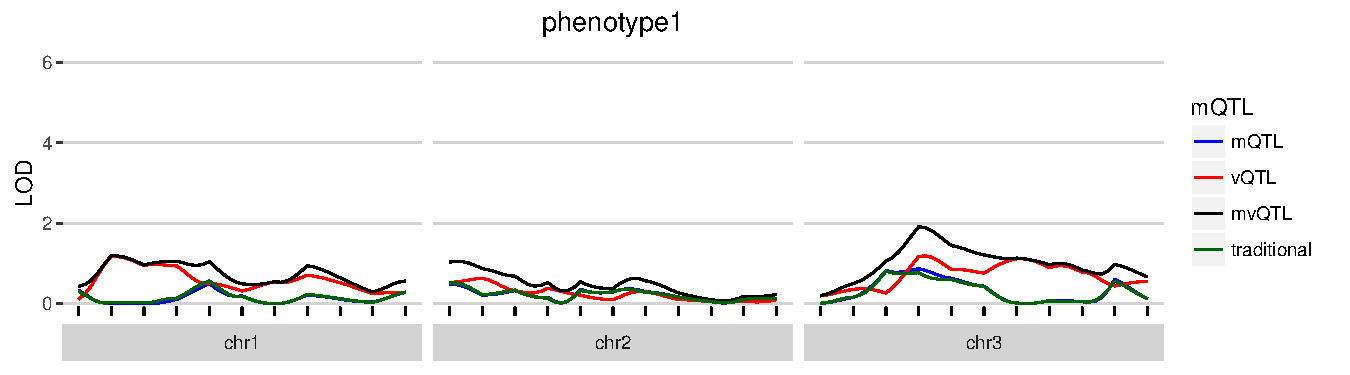
\includegraphics[width=\textwidth]{images/LOD_scan_phenotype1.pdf}
    \end{subfigure}
    \begin{subfigure}[b]{\linewidth}
        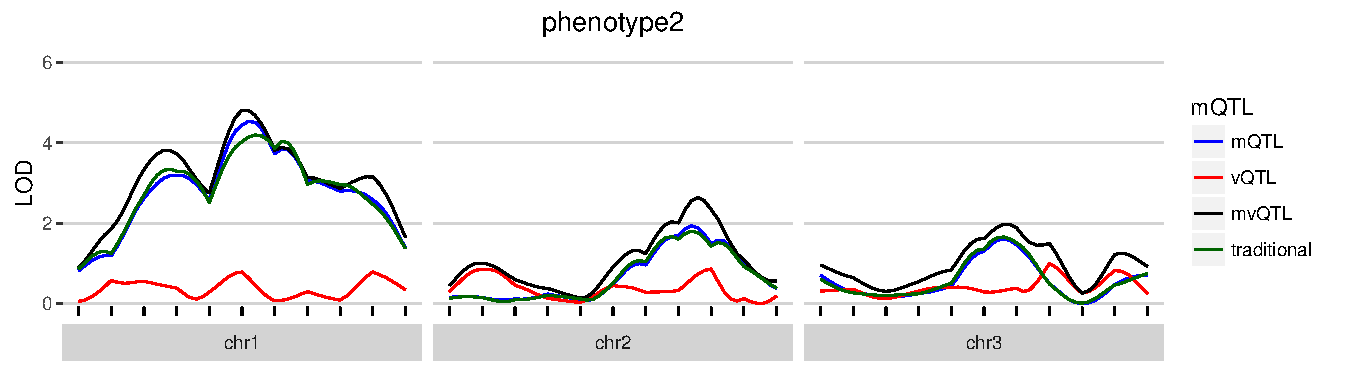
\includegraphics[width=\textwidth]{images/LOD_scan_phenotype2.pdf}
    \end{subfigure}
    \begin{subfigure}[b]{\linewidth}
        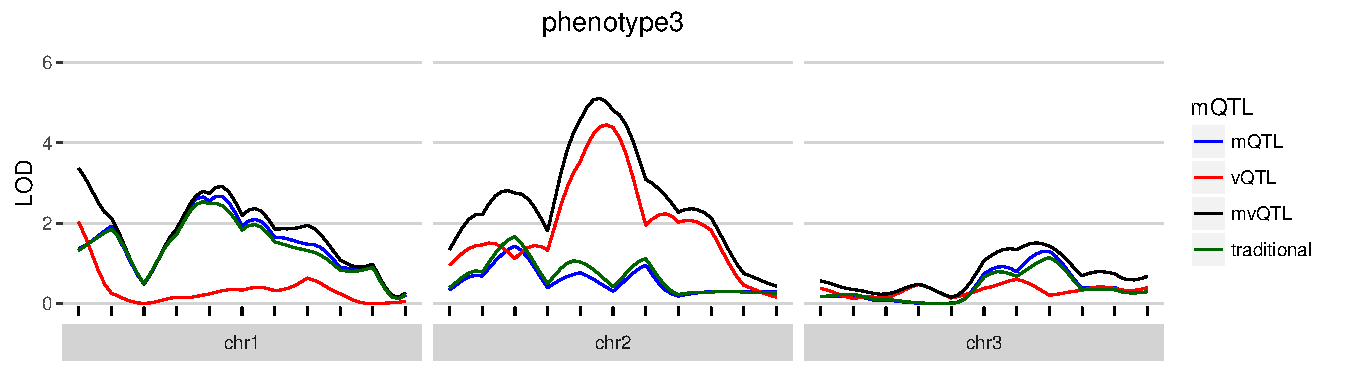
\includegraphics[width=\textwidth]{images/LOD_scan_phenotype3.pdf}
    \end{subfigure}
    \begin{subfigure}[b]{\linewidth}
        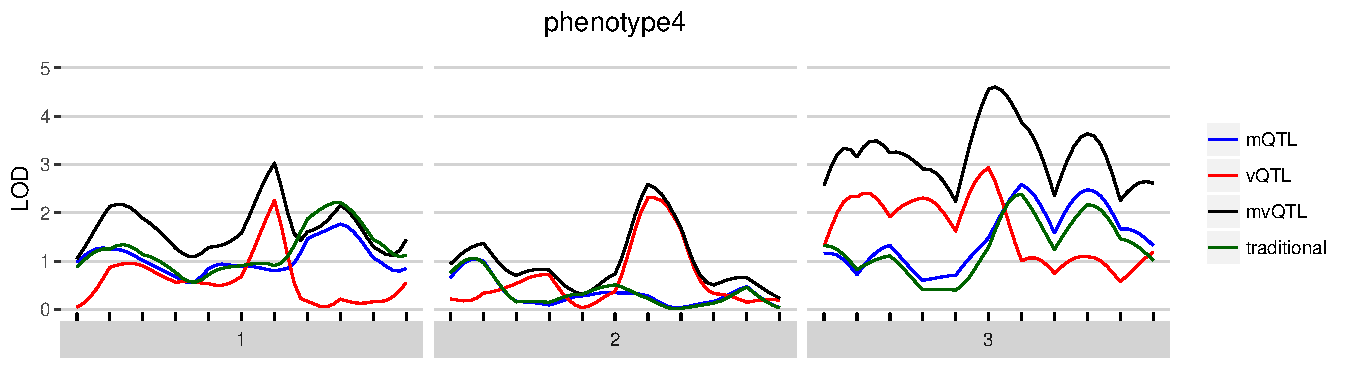
\includegraphics[width=\textwidth]{images/LOD_scan_phenotype4.pdf}
    \end{subfigure}
    \caption{
        For each of the four simulated phenotypes, the genome scan shows the LOD score of each test --- mQTL, vQTL, and mvQTL --- in blue, red, and black, respectively.
        The traditional test is in green and globally similar to the mQTL test.
    }
    \label{fig:lod_score_scans}
\end{figure}

Each type of test (mQTL, vQTL, and mvQTL) yields two association statistics: the LOD score, and the (nominal) $p$-value.
The LOD is a raw measure of association equal to the base 10 logarithm of the likelihood ratio (LR) between the fitted alternative and null models.
Higher values indicate greater association when considered across loci for the same type of test; but LOD scores between different types of tests, namely between mvQTL test vs either mQTL or vQTL tests, are not readily comparable.
The $p$-value, which is comparable between different types of tests, transforms the LOD score to take account of the number of parameters being fit: it is calculated from the asymptotic distribution of $2\log_e\left(\text{LR}\right)$ under the null model, namely the $\chi^2$ distribution with degrees of freedom equal to the difference in the number of parameters between the alternative and null models.
% With this example dataset, it takes five seconds to run one genome scan on a Intel Core i5.

The $p$-values described above, however, are nominal: they do not take into account multiple testing across the genome.
\RC{
    They also rely on asymptotic theory that assumes the underlying phenotype being residually normal; this may not always be the case and when violated will lead to inflated significance.
}{
    Could change this to read ``They also rely on the alternative model being exactly true; severe model misspecification is severe this can lead to inflated statistics.''
    Would be more accurate, but I don't know the rules with regards to things the reviewer didn't mention.
}

More robust $p$-values that are corrected for genomewide significance via control of the family-wise error rate (FWER) can be obtained empirically, through a permutation procedure described below.

\subsection{Robust, genomewide-adjusted p-values}

\begin{figure}[t]
    \begin{subfigure}[b]{\linewidth}
        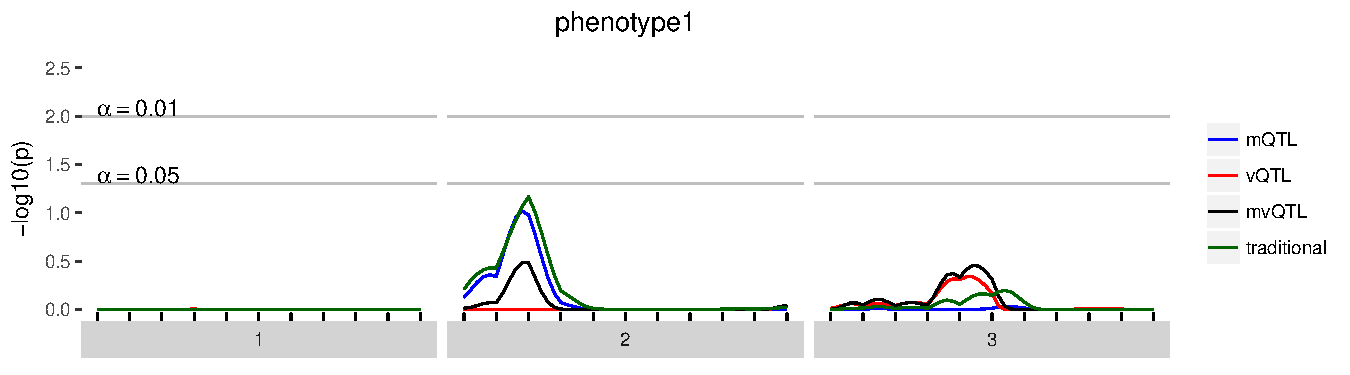
\includegraphics[width=\textwidth]{images/empir_p_scan_phenotype1.pdf}
    \end{subfigure}

    \begin{subfigure}[b]{\linewidth}
        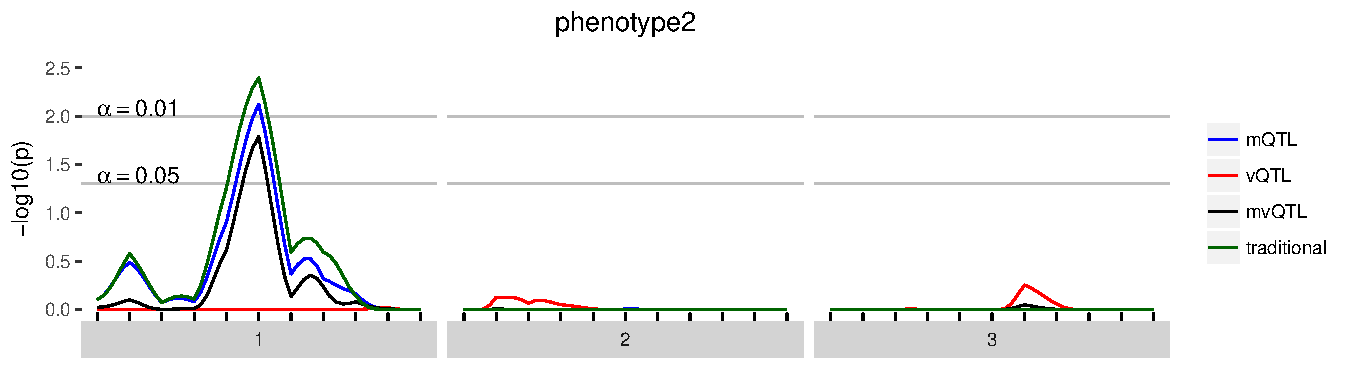
\includegraphics[width=\textwidth]{images/empir_p_scan_phenotype2.pdf}
    \end{subfigure}

    \begin{subfigure}[b]{\linewidth}
        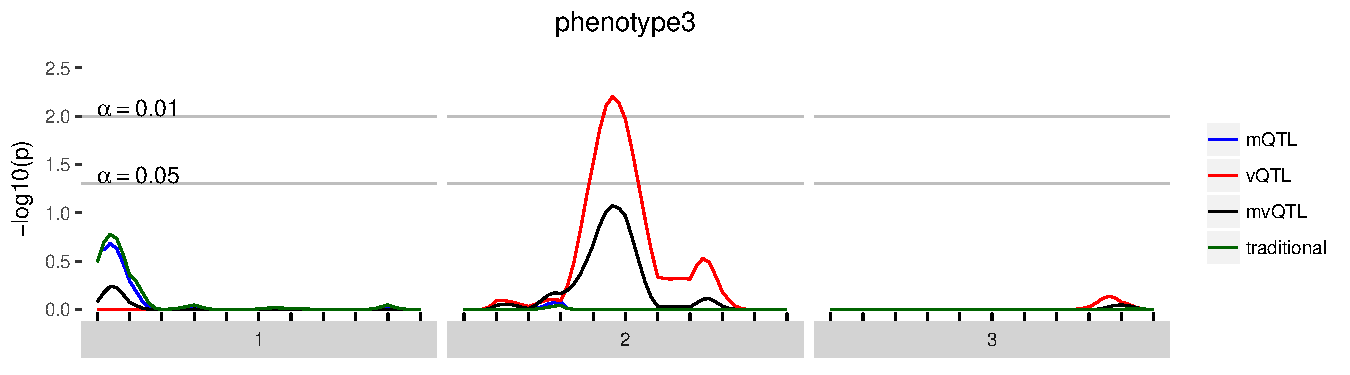
\includegraphics[width=\textwidth]{images/empir_p_scan_phenotype3.pdf}
    \end{subfigure}

    \begin{subfigure}[b]{\linewidth}
        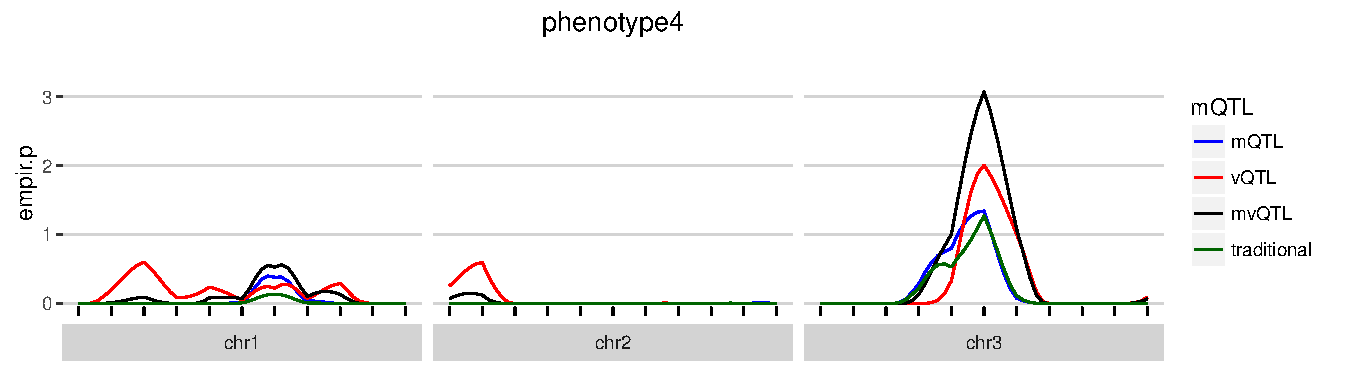
\includegraphics[width=\textwidth]{images/empir_p_scan_phenotype4.pdf}
    \end{subfigure}

    \caption{
        For each of the four simulated phenotypes, the genome scan shows the -log10 of the FWER-corrected $p$-value for each test --- mQTL, vQTL, and mvQTL --- in blue, red, and black, respectively.
        The traditional test is in green and globally similar to the mQTL test.
        A value of 2 implies that the quantity of evidence against the null is such that we expect to see this much or more evidence once per hundred phenotypes no QTL.
    }
    \label{fig:empir_p_scans}
\end{figure}

To calculate the empirical, FWER-controlled $p$-value of each test at each locus we advocate use of a permutation procedure [\CortyMethodsPaper].
Like previous work on permutation-based thresholds for genetic mapping \citep{Churchill1994,Carlborg2002}, this procedure sidesteps the need to explicitly estimate the effective number of tests.

In brief, this approach involves conducting many genomes scans on pseudo-null data generated through permutation to maintain as much of the character of the data as possible, while breaking the tested phenotype-genotype association.
Specifically, the design matrix of the QTL is permuted in the mean portion of the mQTL alternative model, the variance portion of the vQTL alternative model, and in both portions of the mvQTL alternative model.

For each test (mQTL, vQTL, and mvQTL), the highest observed test statistic is extracted from each permutation scan and the collection of statistics that results is used to fit a generalized extreme value (GEV) density \citep{Stephenson2002,Dudbridge2004,Valdar06cc}.
The observed LOD scores from the genome scan are then transformed by the cumulative distribution function of the extreme value density to estimate the FWER-controlling $p$-values.
This approach is implemented in the function, \texttt{scanonevar.perm}, which requires two inputs:
\begin{enumerate}
	\item \texttt{sov} is the \texttt{scanonevar} object, the statistical significance of which will be assessed through permutation.
	\item \texttt{n.perms} is the number of permutations to conduct.
\end{enumerate}
The object returned by \texttt{scanonevar.perm} is a \texttt{scanonevar} object with two additional pieces of information: an empirical $p$-value for each test at each locus and the per-permutation maxima that were used to calculate those $p$-values.
These FWER-corrected $p$-values are straightforwardly interpretable: $p = 0.05$ for a specific test at a specific locus implies that in 5\% of similar experiments where there is no true genotype-phenotype association, we would expect to observe some locus with this much or more evidence of association in this test.
% Additionally, the returned object contains a list of the per-genome-scan maximum observed LOD for each test and each chromosome type.

Accurate estimation of the FWER-controlled $p$-values requires many permutation scans: traditionally recommended is 1,000 (\eg, \citealt{Churchill1994,Carlborg2002}), although the efficiency gain of using the GEV rather than raw quantiles means that fewer may be adequate in practice \citep{Valdar06cc}.
These permutation scans can be run on multiple processors by specifying the optional \texttt{n.cores} argument, which defaults to the total number of cores on the computer minus 2.
On an Intel Core i5, running 100 permutations on this dataset takes about five minutes.
When many phenotypes are studied, or if faster runtimes are needed, these permutation scans can be broken into groups with different values for \texttt{random.seed}, run on separate computers, and combined with the \texttt{c} function.
This function combines the permutations from all the inputted scans, re-estimates the extreme value density, re-evaluates the observed LOD scores in the context of new extreme value density, and returns a new \texttt{scanonevar} object with more precisely estimated empirical $p$-values.

\subsection*{Reporting and plotting genome scans}

The results of \texttt{scanonevar} can be plotted by calling \texttt{plot} on the \texttt{scanonevar} output object. This produces a publication-quality figure that shows the association of the phenotype for each location in the genome as different colors for type of test, with y-axis scale being specified by the user, via option \texttt{plotting.units} as the LOD (\autoref{fig:lod_score_scans}), nominal $p$-value, or, provided permutations have been run, empirical, FWER-controlling $p$-value (\autoref{fig:empir_p_scans}). Of the available y-axis scales, we recommend using the FWER-controlled $p$-values since this scale puts all tests on a level-footing (unlike the LOD), and allows direct identification of genomewide significance and thereby relevance (unlike the nominal $p$-value).

Calling \texttt{summary} on the output of \texttt{scanonevar} produces a summary of how the scan was conducted and what the results were.

% The details of the null and alternative models used in each of the three tests can be found in the companion article [CompanionC].

% The object returned by the \texttt{scanonevar} function has class \texttt{scanonevar}.
% Calling \texttt{plot} on this object produces a publication-quality plot that shows the three association statistics at each locus.

% \subsection*{The LOD Score --- Problems and an Alternative}
% \WV{}{Edits to here so far}
% QTL mapping in model organisms is traditionally reported via the LOD score. However, for reporting the results of mean-variance QTL mapping, the LOD score is cumbersome because it is not comparable across tests with different degrees of freedom; in this case, the mvQTL test has twice as many degrees of freedom as the mQTL or vQTL tests, meaning that each type of test needs to be presented with its own threshold.

% (2) Another problem with the LOD score is that it relates only to a single locus.
% Geneticists must take into account the many hypotheses that are tested.
% When a significance threshold is established, \eg by permutation, to control family-wise error rate, it divides 

% (1) It must be interpreted differently in autosomes and sex chromosomes.
% The sex chromosomes are typically fit with fewer parameters, depressing the expected value of the LOD scores under the null, and thus increasing the significance of any observed LOD score.
% (2) It's interpretation depends on which test was conducted -- mQTLLOD scores from different tests must be interpreted differently.
% For example, the LOD score of the mvQTL test is always higher than the LOD score of the mQTL and vQTL tests.
% This relationship is due to the nested nature of the mvQTL test and the other two tests, where they all share an alternative model and the mvQTL test uses a null model that combines the restrictions of the mQTL null and vQTL null.
% (3) It relates only to a single locus.

% All three tests use the same alternative model, but the null model in the mvQTL test imposes all the constraints of the null of the mQTL test and all the constraints of the null of the vQTL test, so the LOD score of the mvQTL test must, by definition, be greater than the LOD score of the other tests.

% These difficulties in interpreting the LOD score are evident in \autoref{fig:lod_score_scans}.
% It seems that there are no important signals in the genome scan of \texttt{phenotype1} and it is visually clear that the most interesting signals for \texttt{phenotype2}, \texttt{phenotype3}, and \texttt{phenotype4} are on chromosomes one, two, and three, respectively.
% But important questions remain:
% (1) If we didn't have the genome scans from \texttt{phenotype2} -- \texttt{phenotype4} available for comparison, would we be confident there are no statistically significant signals related to \texttt{phenotype1}?
% (2) How can we compare the results of the mvQTL test to the results of the other tests?
% (3) How could we compare the results of tests on autosomes to tests on sex chromosomes (if they were present)?
% (4) How often do we expect to observe results of this magnitude or greater when there is no true association, due simply to sampling variation and the multiplicity of tests conducted?

% To put all genetic loci and all three tests on a level playing field, we consider two types of $p$-values:
% (1) Asymptotic $p$-values are calculated by \texttt{scanonevar} using the $\chi^2$ distribution with the appropriate degrees of freedom for each locus.
% Though these $p$-values overcome the questions 1 through 3 of working with LOD scores described above, they leave question 4 unresolved.
% (2) Empirical, family-wide error rate (FWER)-corrected $p$-values resolve all the above questions with interpreting LOD scores so they are our preferred association statistics in most cases.
% % thus they are the recommended means of assessing the significance of QTL mapping results.
% % Statistical methods for empirical FWER control in mean-variance QTL mapping are described in \CortyMethodsPaper.



%\section*{Assess the Significance of Results}


% The $p$-value assigned to each locus by calculating the position of its calculated LOD score in its null distribution answers the question, ``How probable is it to observe this much of a deviation from the null at this locus, given that there is no true effect?''
% This question is not entirely relevant for genetic mapping, however, because we typically test for association at many loci, with no special interest in any individual locus \textit{a priori}.
% Thus, a more appropriate $p$-value would answer the question, ``How probable is it to observe this much or more deviation from the null at \textit{some} locus in the genome, given that there are no true effects?''
% This is precisely the reasoning behind the family-wide-error-rate (FWER) controlling procedure we illustrate below.

% To calculate a FWER-controlling $p$-value, one typically must estimate the effective number of statistical tests conducted.
% The effective number of tests in a genome scan, however, is difficult to estimate.
% One lower bound is the number of chromosomes.
% Due to the randomization in meiosis no two non-syntenic loci are correlated in an experimental cross and therefore tests on different chromosomes are always independent.
% But there are many non-identical tests conducted on each chromosome, so the number of chromosomes is an under-estimate.
% One upper bound on the effective number of tests is the total number of loci.
% But, loci on the same chromosome are often in linkage disequilibrium, therefore the tests are not independent and the total number of loci is an over-estimate \citep{Lander1989a}.


\section*{Communicate Significant Findings}

\begin{figure}[t]
    \begin{subfigure}[t]{0.5\linewidth}
        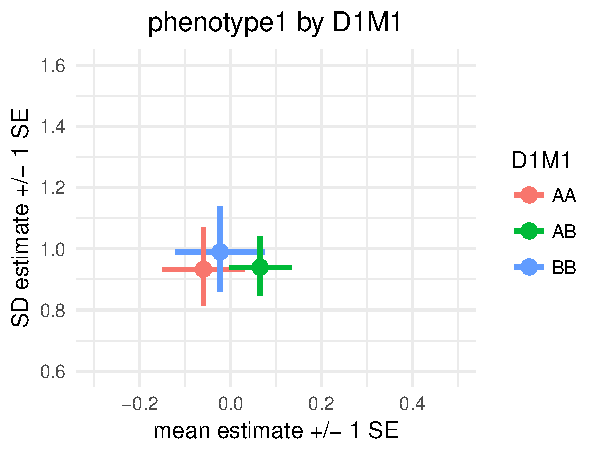
\includegraphics[width=\textwidth]{images/mean_var_plot_phen1.pdf}
    \end{subfigure}
    \hfill
    \begin{subfigure}[t]{0.5\linewidth}
        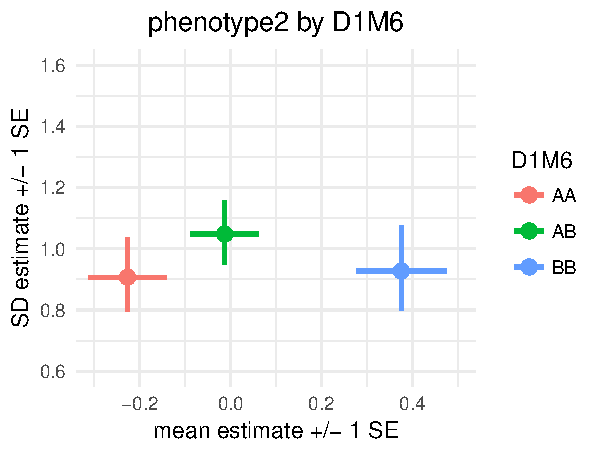
\includegraphics[width=\textwidth]{images/mean_var_plot_phen2.pdf}
    \end{subfigure}

    \begin{subfigure}[t]{0.5\linewidth}
        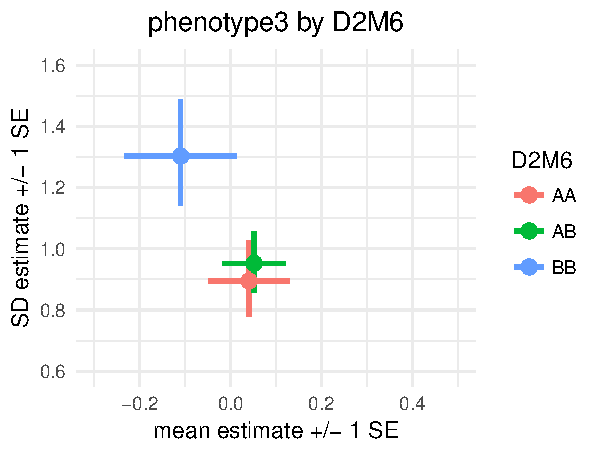
\includegraphics[width=\textwidth]{images/mean_var_plot_phen3.pdf}
    \end{subfigure}
    \hfill
    \begin{subfigure}[t]{0.5\linewidth}
        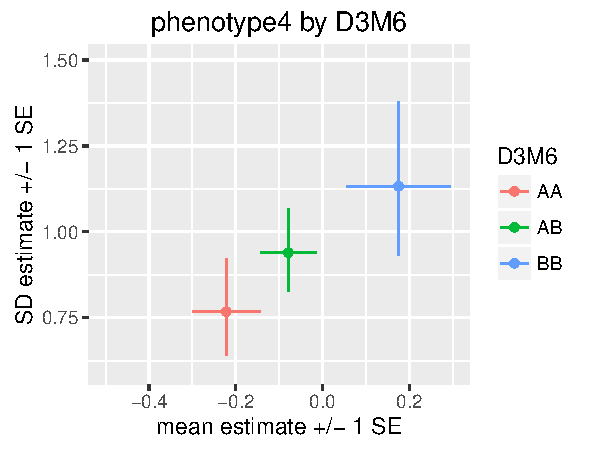
\includegraphics[width=\textwidth]{images/mean_var_plot_phen4.pdf}
    \end{subfigure}

    \caption{
        \texttt{mean\_var\_plot}s show the estimated genotype effects at a locus with mean effects on the horizontal axis and variance effects on the vertical axis.
        Horizontal lines indicate standard errors for mean effects and vertical lines indicate standard errors for variance effects.
        For \texttt{phenotype1}, the pattern of overlapping estimates and standard errors is consistent with the fact that there are no genetic effects, and the $p$-value was not statistically significant at any locus.
        For \texttt{phenotype2}, the pattern of horizontal, but not vertical, separation visually illustrates the identified mQTL.
        For \texttt{phenotype3}, the pattern of vertical, but not horizontal, separation visually illustrates the identified vQTL.
        For \texttt{phenotype4}, the pattern of two-dimensional separation illustrates an mvQTL.
        \label{fig:mean_var_plots}
    }
\end{figure}

Having identified interesting QTL, we want to visualize the their estimated genetic and covariate effects.
Because the \texttt{vqtl} package models effects for both mean and variance, existing plotting utilities are not able to display the entirety of the modeling results.
To understand and communicate the results of a \texttt{vqtl} scan at one particular locus, we developed the \texttt{mean\_var\_plot}.
This plot illustrates how the mean sub-model and variance sub-model of the DGLM fit the data at a given locus.

In each \texttt{mean\_var\_plot} in \autoref{fig:mean_var_plots}, the location of the dot shows the estimated mean and standard deviation of each genotype group, with the mean indicated by the horizontal position and the standard deviation indicated by the vertical position.
The horizontal lines extending to the left and right from each dot show the standard error of the mean estimate, and the vertical lines extending up and down from each dot show the standard error of the standard deviation estimate.
There are two types of grouping factors considered by the function \texttt{mean\_var\_plot\_model\_based}:
(1) \texttt{focal.groups} are groups that are modeled and the prediction for each group is plotted.
For example, a genetic marker is the \texttt{focal.group} in each plot in \autoref{fig:mean_var_plots}; \texttt{D1M1} in the top left, \texttt{D1M6} in the top right, \texttt{D2M6} in the bottom left, and \texttt{D3M6} in the bottom right.
(2) \texttt{nuisance.groups} are groups that are modeled, but then averaged over before plotting.
When there are many grouping factors thought to play a role in determining the mean and variance of an individual's phenotype, such as sex, treatment, and batch, we recommend putting just one or two in \texttt{focal.groups} and the others in \texttt{nuisance.groups} for clarity, cycling through which are displayed to gain a thorough understanding of the factors that influence the phenotype.


% The identification of an mQTL is consistent, roughly speaking, with horizontal distances between genotype groups that exceed the horizontal standard error bars.
% The identification of a vQTL is consistent with vertical distances between genotype groups that exceed the vertical standard error bars.
% And the identification of an mvQTL is consistent with euclidean distance between genotype groups that exceed the standard error density implied by both the horizontal and vertical standard errors.

Additional plotting utilities, \texttt{phenotype\_plot}, \texttt{effects\_plot} and \texttt{mean\_var\_plot\_model\_free} are described in the online documentation, available on CRAN.

\section{Establish a Confidence Interval for the QTL}

Last, it is important to assess the genetic precision of a discovered QTL for bioinformatic follow-up.
The function \texttt{scanonevar.boot} implements the non-parametric bootstrap \citep{Visscher1996}.
This function takes, as arguments, a \texttt{scanonevar} object, the type of QTL detected, the name of the chromosome containing the QTL, and \texttt{num.resamples}, the number of bootstrap resamplings desired.
As with \texttt{scanonevar.perm}, the \texttt{n.cores} argument can be used to spread the bootstraps over many computational cores and defaults to the number of cores available minus two, and bootstraps can be run on separate computers and combined with \texttt{c} to increase the precision of the estimate of the confidence interval.

We recommend 1000 resamples to establish 80\% and 90\% confidence intervals.
With the datasets simulated here, it takes 20 minutes to run 1000 bootstrap resamples on an Intel core i5.


% \section*{Mathematical Details}

% [todo]

% mean-var plot what is on x what is on y and how are SE's calculated

% DGLM with other links and distribs

\section*{Performance Benchmarks}


\begin{figure}[t]
    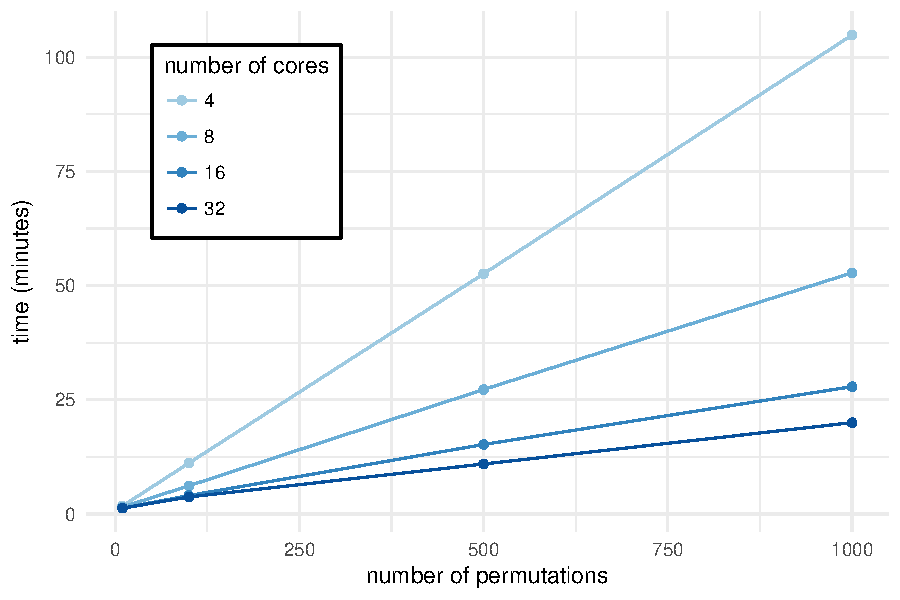
\includegraphics[width = \linewidth]{images/benchmark_kumar.pdf}
    \caption{
        Time taken to run \texttt{scanonevar.perm} on the data from \citet{Kumar2013} which contains 244 individuals and 582 loci, varying the number of permutations desired and the number of computer cores used.
        For a given number of cores, there is a linear relationship between number of permutations conducted and time required.
        The slope the the line indicates time required per permutation and is dependent on the number of cores, ranging from $\approx$ 6.3 seconds per permutation with 4 cores to $\approx$ 1.2 second per permutation with 32 cores.
    }
    \label{fig:benchmark_kumar}
\end{figure}

\begin{figure}[t]
    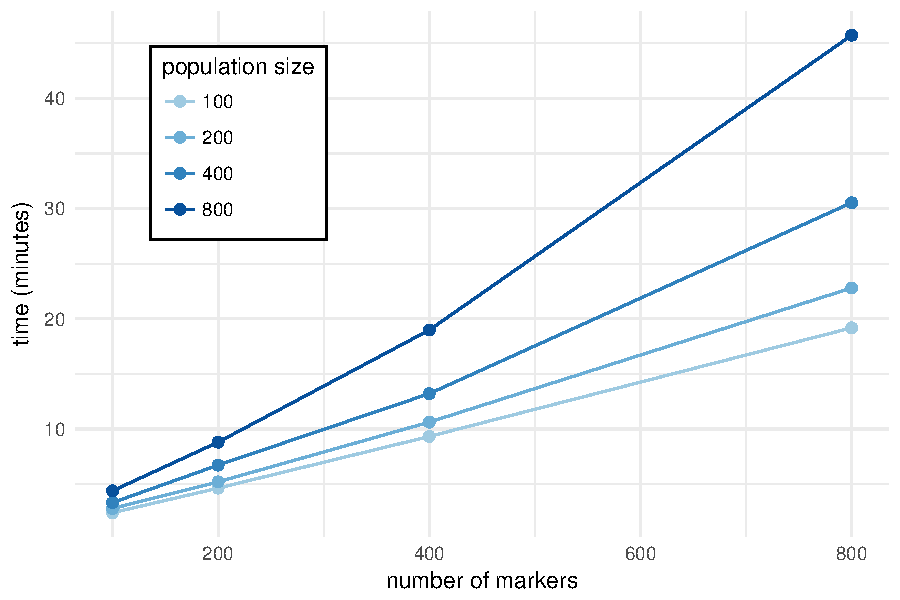
\includegraphics[width = \linewidth]{images/benchmark_sim_cross.pdf}
    \caption{
        Time taken to run 1000 permutation scans on 32 cores on simulated data using \texttt{scanonevar.perm}, varying the number of individuals in the mapping population and the number of markers in the genome.
        For a given population size, there is a slightly supra-linear relationship between number of markers and time required.
        The average slope of the line indicates the average time required per locus and is dependent on the population size, ranging from $\approx$ 1.4 seconds per locus with a population of size 100 to $\approx$ 3.3 seconds per locus with a population of size 800.
    }
    \label{fig:benchmark_sim_cross}
\end{figure}

By far, the most computationally-intensive step in the mean-variance QTL mapping process is the assessment of genome-wide statistical significance by permutation.
The original genome scan is much faster, because it involves only a single scan, and the bootstrap is much faster because it involves only a single chromosome.

For the first benchmark, we ran \texttt{scanonevar.perm} on the data from \citet{Kumar2013} and \CortyReanalysisPaper, which contains 244 individuals and 582 loci, varying the number of permutations desired and the number of computer cores used.
For a given number of cores, there is a linear relationship between number of permutations conducted and time required \autoref{fig:benchmark_kumar}.
The slope the the line indicates time required per permutation and is dependent on the number of cores, ranging from $\approx$ 6.3 seconds per permutation with 4 cores to $\approx$ 1.2 second per permutation with 32 cores.

For the second benchmark, we ran \texttt{scanonevar.perm} on simulated data, always conducting 1000 permutations and using 32 cores, but varying the number of individuals in the mapping population and the number of markers in the genome.
For a given population size, there is a slightly supra-linear relationship between number of markers and time required \autoref{fig:benchmark_sim_cross}, which reflects a linear increase in the time taken to conduct the permuted genome scans, plus an increase in the time taken for ``bookkeeping'' tasks like organizing and reshaping genetic data.
The slope of the line indicates the time required per locus and is dependent on the population size, ranging from $\approx$ 1.4 seconds per locus with a population of size 100 to $\approx$ 3.3 seconds per locus with a population of size 800.

Based on these benchmarks, it is clear that the workflow presented here is practical for QTL mapping F2 intercross and similar populations on modern, multi-core scientific computers.
Populations with many recombinations, where dense genotyping arrays that interrogate $\textgreater$ 10,000 loci are relevant, could not be practically analyzed with package \texttt{vqtl} in this way.
\RC
{
    \WV
    {
        However, both statistical and computational steps could be taken to make such a study feasible.
    }{
        Are there ways to make efficient the analysis of multiple traits on the same population? For example, in the standard analysis of gene expression data, rint-ing a probe then performing permutations on it provides thresholds that will be valid for all other rint-ed probes (assuming no missingness; eg, ask Greg). Not sure if this applies in our situation... needs more thought.
    }
}
{
    I think simply suggesting that larger-scale analysis might be possible is appropriate here, since we haven't done it and haven't even worked out how to do it.
    I don't think it makes sense for us to try to figure out how we would have done a different study and report exactly how we would have done that.
}
Statistically, techniques could be used that allow for large-scale analysis without permutation testing \citep{Efron2004}.
Computationally, the software could be changed to run on a computer cluster, rather than on a single computer \citep{Jette2003a,Marchand2017}.
\RC
{
    \WV{}
    {Does this section extend the paper beyond the required limits.}
}
{
    Yes.  Do you think they will notice/care?
}

% Performance benchmarks of package \texttt{vqtl} are presented in \autoref{fig:benchmark_kumar} and \autoref{fig:benchmark_sim_cross}.

% \begin{table}
%     \centering
%     \begin{tabular}{r|rrrr}
%         \multirow{2}{1in}{\raggedleft \textbf{number of permutations}}& \multicolumn{4}{c}{\textbf{number of cores}}\\
%         \cline{2-5}
%         & 4 & 8 & 16 & 32\\
%         \hline
%         100  & 11 & 6 & 4 & 4\\
%         1000 & -  & 53 & 34 & 20\\
%         \hline
%     \end{tabular}
%     \caption{
%         Time in minutes required to conduct permuations for all three tests on the dataset from \citet{Kumar2013}, which has 244 individuals and 582 loci, according to number of permutations desired and number of computer cores available.
%         We recommend 1000 permutations for publication-quality precision.
%         We include the time taken to conduct 100 and 500 permutations to illustrate the linear relation between number of permutations and time required.
%         This table also illustrates the linear relationship between number of computer cores used and time taken to complete permutations.
%     }
% \end{table}
%
% \begin{table}
%     \centering
%     \begin{tabular}{r|rrrr}
%         \multirow{2}{1in}{\raggedleft \textbf{number of markers}}& \multicolumn{4}{c}{\textbf{number of individuals}}\\
%         \cline{2-5}
%         & 100 & 200 & 400 & 800\\
%         \hline
%         100 & 2 & 3 & 4 & 4\\
%         200 & 5 & 5 & 7 & 9\\
%         400 & 9 & 11 & 13 & 19\\
%         800 & 19 & 23 & 31 & 46\\
%         \hline
%     \end{tabular}
%     \caption{Time in minutes required to conduct 1000 permuations on 32 cores for all three tests on a simulated F2 intercross, according to number of individuals in the mapping population and number of markers in the genome.}
% \end{table}

\section*{Conclusion}

We have demonstrated typical usage of the \texttt{R} package \texttt{vqtl} for mean-variance QTL mapping in an F2 intercross.
This package is appropriate for crosses and phenotypes where genetic factors or covariates or are known or suspected to influence phenotype variance.
In the case of genetic factors, they can be mapped, as illustrated in one companion article (\CortyReanalysisPaper).
In the case of covariates, they can be accommodated, which can increase power and improve false positive rate control, as illustrated in another companion article (\CortyMethodsPaper).

\section*{Resources}
The scripts used to simulate genotypes and phenotypes, conduct the genome scans, and plot the results are available as a public, static Zenodo repository at \url{DOI: 10.5281/zenodo.1173799}.
The package \texttt{vqtl} and its documentation are freely available on \texttt{CRAN} at \url{https://CRAN.R-project.org/package=vqtl}.

% The central function of this package, \texttt{scanonevar}, carries out the initial genome scan.
% The permutation function, \texttt{scanonevar.perm}, executes a set of permutations to empirically estimate a FWER-controlling $p$-value for each observed LOD score.
% A suite of plotting functions, e.g. the \texttt{mean\_var\_plot}, allows geneticists to evaluate the allelic and covariate effects that underlie detected signals.
% The bootstrap function, \texttt{scanonevar.boot}, executes bootstrap resampling to assess the genetic precision of a QTL and extablish a confidence interval. 

\section{Acknowledgments}
This work was primarily funded by a National Institutes of General Medical Sciences (NIGMS) grant to WV (R01-GM104125) and a National Institutes of Mental Health grant to RWC (F30-MH108265).
RWC received additional support from NIGMS grant T32-GM067553 and National Library of Medicine grant T32-LM012420.


\bibliography{10_Aim1,wv}


\clearpage
\newpage
\section*{Appendix}

\setcounter{figure}{0}
\renewcommand{\thefigure}{A\arabic{figure}}

\begin{figure}[ht]
    \begin{subfigure}[b]{\linewidth}
        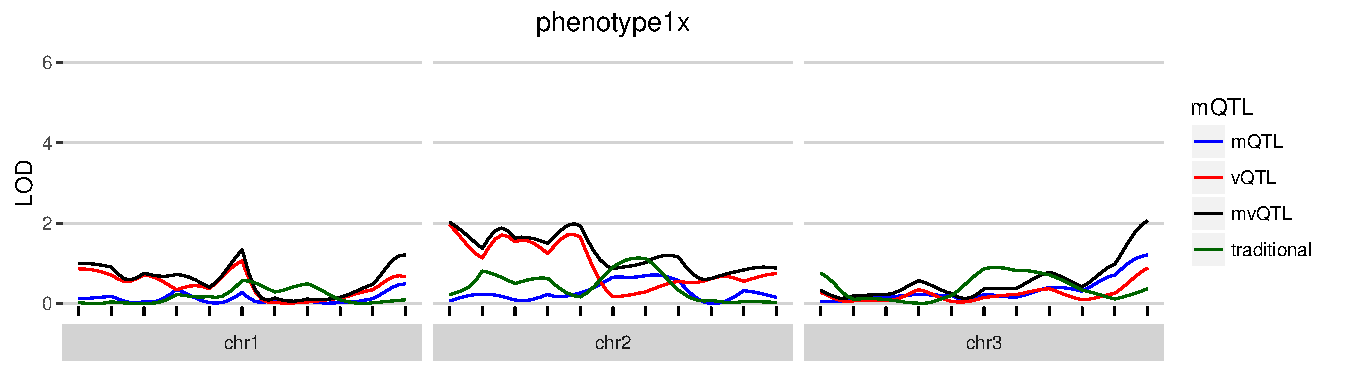
\includegraphics[width=\textwidth]{images/LOD_scan_phenotype1x.pdf}
    \end{subfigure}

    \begin{subfigure}[b]{\linewidth}
        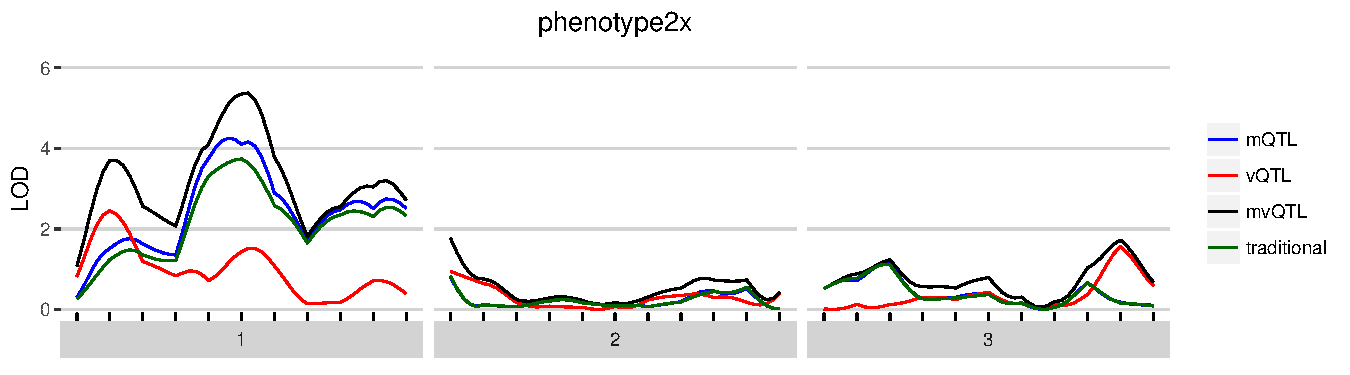
\includegraphics[width=\textwidth]{images/LOD_scan_phenotype2x.pdf}
    \end{subfigure}

    \begin{subfigure}[b]{\linewidth}
        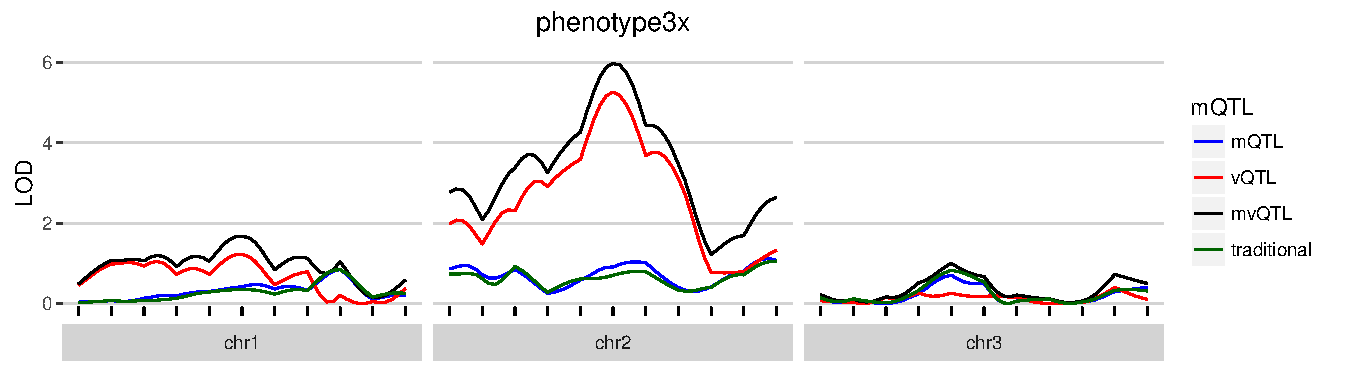
\includegraphics[width=\textwidth]{images/LOD_scan_phenotype3x.pdf}
    \end{subfigure}

    \begin{subfigure}[b]{\linewidth}
        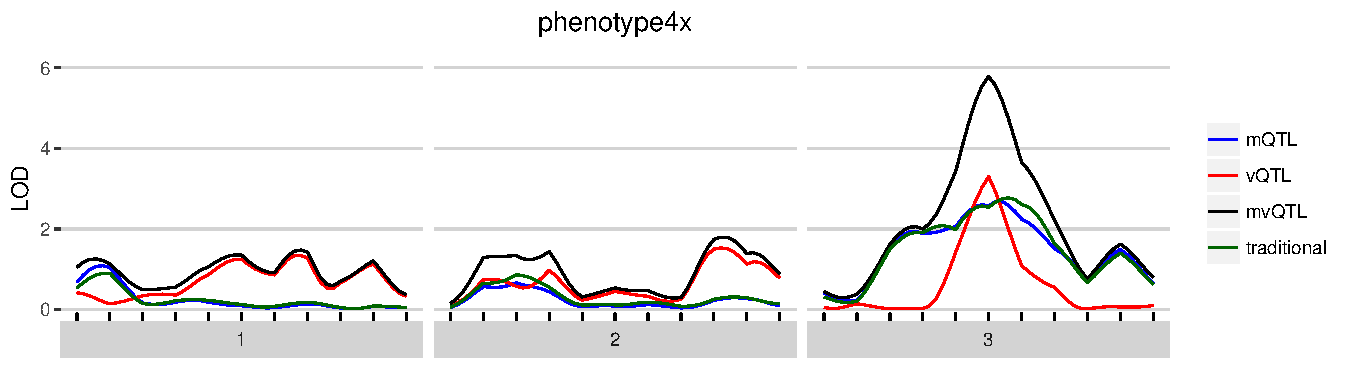
\includegraphics[width=\textwidth]{images/LOD_scan_phenotype4x.pdf}
    \end{subfigure}

    \caption{For each of the four simulated phenotypes with background variance heterogeneity, the genome scan shows the LOD score of each test -- mean, variance, and joint -- in blue, red, and black, respectively.  The traditional test is in green and globally similar to the mean test. \label{fig:apdx_lod_score_scans}}
\end{figure}

\begin{figure}[ht]
    \begin{subfigure}[b]{\linewidth}
        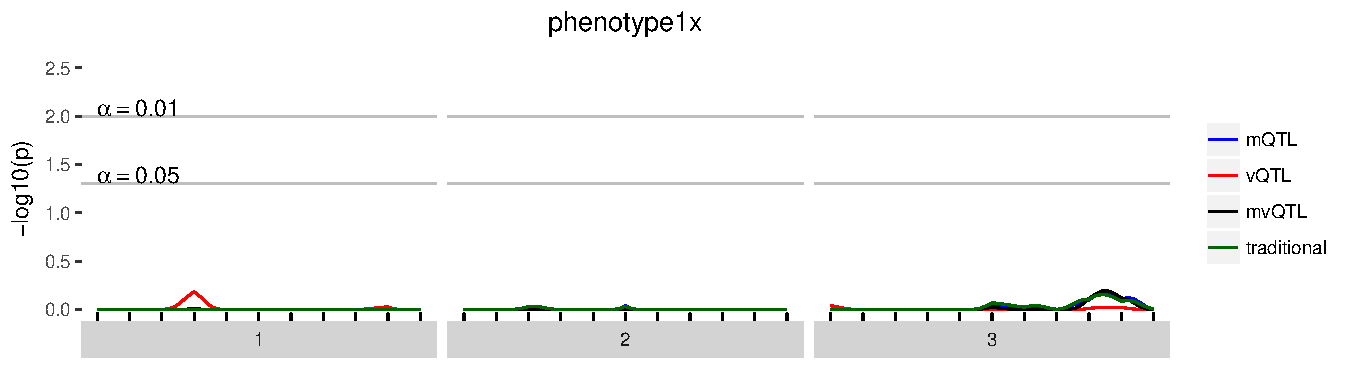
\includegraphics[width=\textwidth]{images/empir_p_scan_phenotype1x.pdf}
    \end{subfigure}

    \begin{subfigure}[b]{\linewidth}
        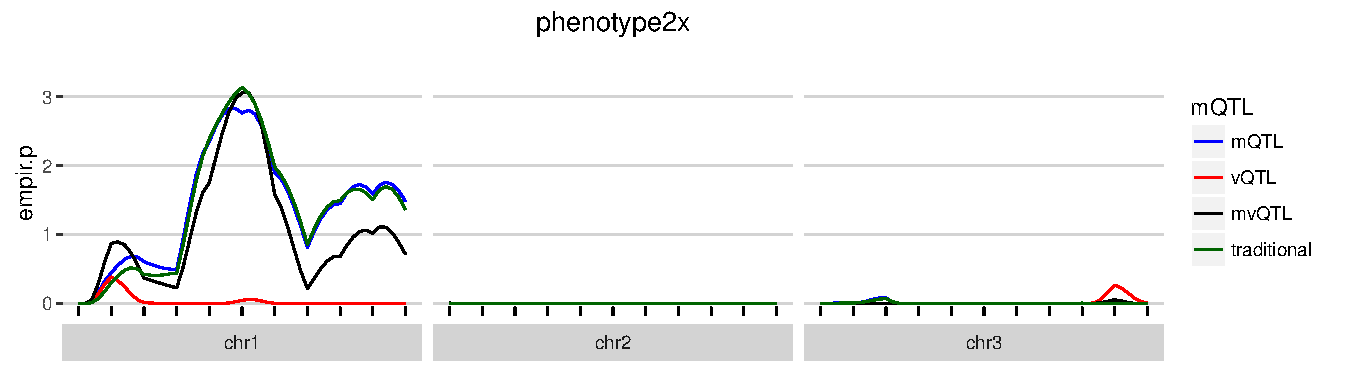
\includegraphics[width=\textwidth]{images/empir_p_scan_phenotype2x.pdf}
    \end{subfigure}

    \begin{subfigure}[b]{\linewidth}
        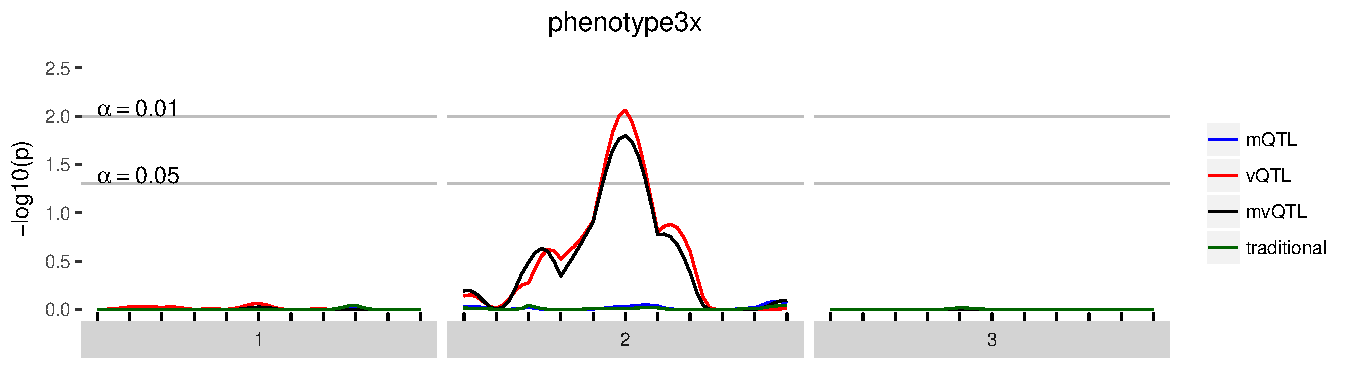
\includegraphics[width=\textwidth]{images/empir_p_scan_phenotype3x.pdf}
    \end{subfigure}

    \begin{subfigure}[b]{\linewidth}
        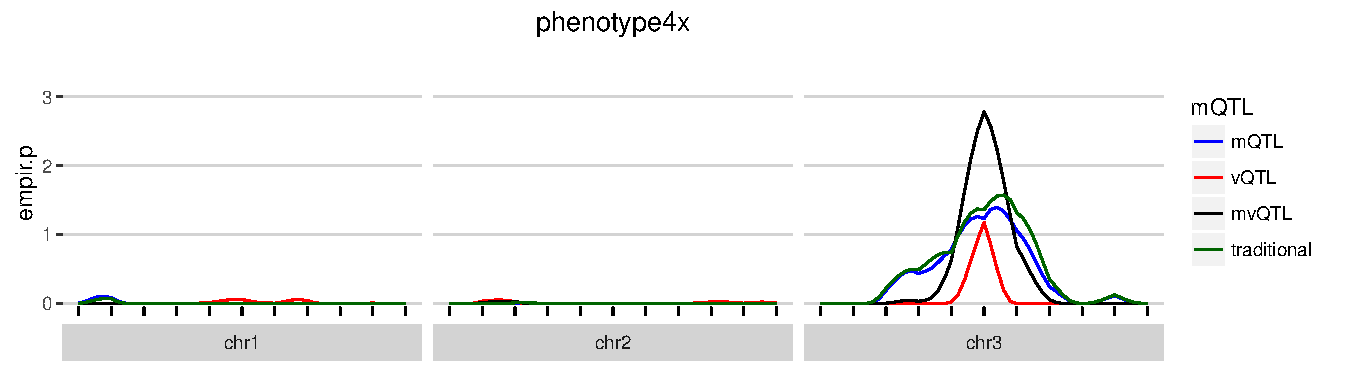
\includegraphics[width=\textwidth]{images/empir_p_scan_phenotype4x.pdf}
    \end{subfigure}

    \caption{For each of the four simulated phenotypes with background variance heterogeneity, the genome scan shows the -log10 of the FWER-corrected $p$-value of each test -- mean, variance, and joint -- in blue, red, and black, respectively. Thus, a value of 3 implies that the quantity of evidence against the null is such that we expect to see this much or more evidence once per thousand genome scans when there is no true effect. \label{fig:apdx_empir_p_scans}}
\end{figure}

\begin{figure}[ht]
    \begin{subfigure}[t]{0.5\linewidth}
        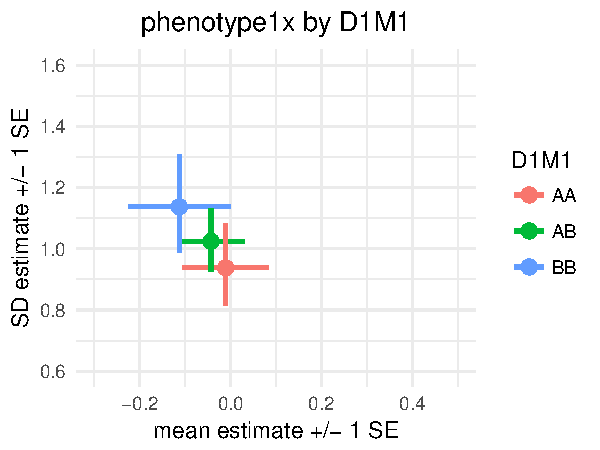
\includegraphics[width=\textwidth]{images/mean_var_plot_phen1x.pdf}
    \end{subfigure}
    \hfill
    \begin{subfigure}[t]{0.5\linewidth}
        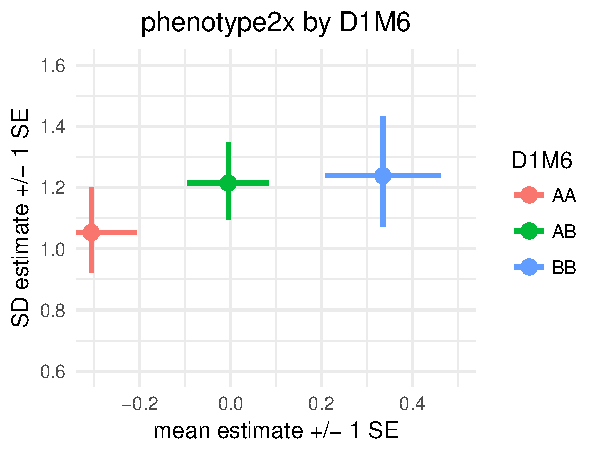
\includegraphics[width=\textwidth]{images/mean_var_plot_phen2x.pdf}
    \end{subfigure}

    \begin{subfigure}[t]{0.5\linewidth}
        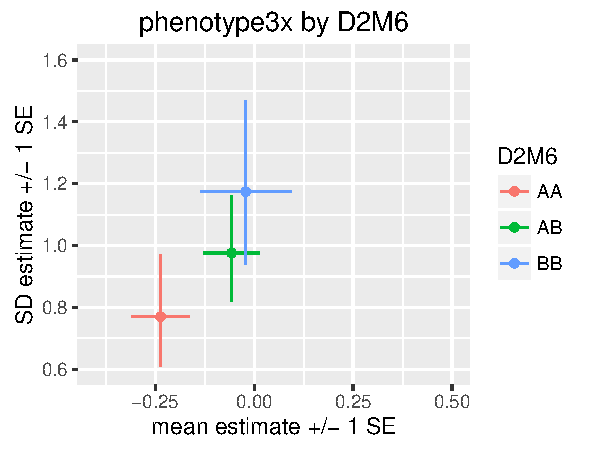
\includegraphics[width=\textwidth]{images/mean_var_plot_phen3x.pdf}
    \end{subfigure}
    \hfill
    \begin{subfigure}[t]{0.5\linewidth}
        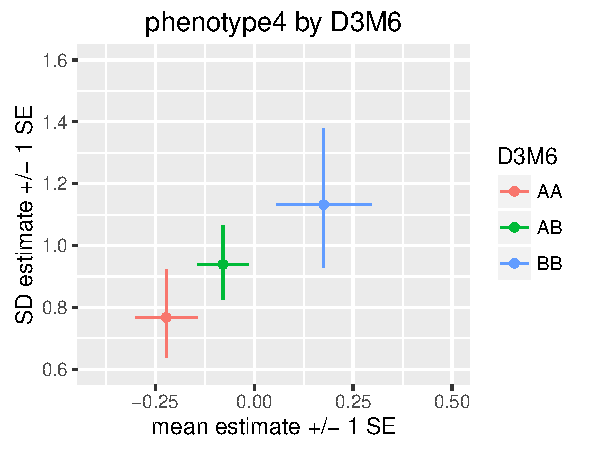
\includegraphics[width=\textwidth]{images/mean_var_plot_phen4x.pdf}
    \end{subfigure}

    \caption{
         \texttt{mean\_var\_plot}s show the estimated genotype effects at a locus, with mean effects on the horizontal axis and variance effects on the vertical axis.
        Horizontal lines indicate standard errors for mean effects and vertical lines indicate standard errors for variance effects.
        For \texttt{phenotype1x}, the pattern of overlapping estimates and standard errors is consistent with the fact that there are no genetic effects, and the $p$-value was not statistically significant at any locus.
        For \texttt{phenotype2x}, the pattern of horizontal, but not vertical, separation visually illustrates the identified mQTL on a background of variance heterogeneity.
        For \texttt{phenotype3x}, the pattern of vertical, but not horizontal, separation visually illustrates the identified vQTL on a background of variance heterogeneity.
        For \texttt{phenotype4x}, the pattern of two dimensional separation without either total horizontal or vertical separation illustrates an mvQTL with neither mean nor variance effect strong enough to define an mQTL or vQTL on a background of variance heterogeneity.
        \label{fig:mean_var_plots_appendix}
    }
\end{figure}

\end{document}